\section{Aufgabe 2}
\label{sec:Aufgabe2}
%\lstinputlisting[language=Python, firstline=15, lastline=21]{plots/plot.py}
\subsection{Teil a)}
Zufallszahlgeneratoren wiederholen sich ab einer gewissen Anzahl an Rechenoperationen.
Die Periodenlänge nennen wir $P$.\\
Für diesen Aufgabenteil wird ein linear-kongruenter Zufallszahlgenerator mit der
Vorschrift
\begin{equation*}
  x_n=(a\cdot x_{n-1}+3)\%1024
\end{equation*}
verwendet. Der Seed $x_0$ wurde für Aufgabenteil a) gleich Null gewählt.
Dabei wurde der Multiplikator $a$ auf einem Bereich von $0-80$ untersucht.
In der Abbildung \ref{fig:Periodenlaenge} ist die Periodenlänge in Abhängigkeit
des Multiplikators $a$ dargestellt.
\begin{figure}[H]
  \centering
  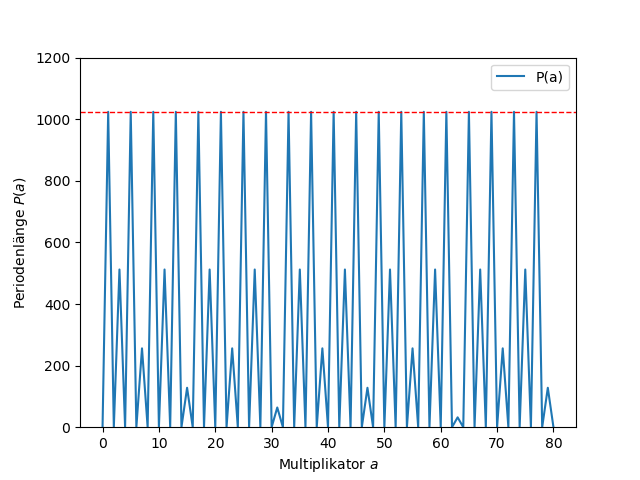
\includegraphics[width=0.6\textwidth]{plots/Periodenlaenge.png}
  \caption{Darstellung der Periodenlänge in Abhängigkeit des Multiplikators.}
  \label{fig:Periodenlaenge}
\end{figure}
Die theoretisch maximale Periodenlänge entspricht dem Modulus, hier $m=1024$.
Diese Periodenlänge wird auch erreicht.\\
In Abbildung \ref{fig:Periodenlaenge} ist die maximale Periodenlänge
eingezeichnet. Die Werte für $a$ bei denen $P$ maximal ist, sind:
\begin{equation*}
  1,5,9,13,17,21,25,29,33,37,41,45,49,53,57,61,65,69,73,77
\end{equation*}
Um eine maximale Periodenlänge zu erreichen müssen folgende Punkte gelten:
\begin{itemize}
  \item $b$ $\neq$ 0
  \item $b$ und $m$ sind teilerfremd
  \item jeder Primfaktor von $m$ teilt $(a-1)$
  \item wenn $m$ durch 4 teilbar ist, ist es auch $(a-1)$
\end{itemize}
Bei der hier verwendeten Wahl von $b$ und $m$ sind die ersten beiden Punkte erfüllt.
Um den nächsen Punkt zu überprüfen, wird eine Primfaktorzerlegung von $m$ gesucht.
Da
\begin{equation*}
  m=1024=2^{10}
\end{equation*}
eine Zweierpotenz ist und nach dem Fundamentalsatz der Arithmetik die Eindeutigkeit
der Primfaktorzerlegung sichergestellt ist, ist 2 der einzige Primfaktor.
Alle Werte für $a$, bei den die Periodenlänge maximal ist, sind ungerade, das heißt,
dass $(a-1)$ durch 2 teilbar ist. Damit ist auch der dritte Punkt erfüllt.
Für den vierten Punkt: $1024/4=256$ und für $(a-1)$ gilt:
\begin{equation*}
  1,2,3,4,5,6,7,8,9,10,11,12,13,14,15,16,17,18,19
\end{equation*}
und damit bis auf $(a-1)=0$ auch durch 4 teilbar.\\
Also können die Ergebnisse mit den Regeln für \textit{gute} linear-kongruente
Generatoren erklärt werden.
\subsection{Teil b)}
Es wurden 10000 Zufallszahlen nach der Vorschrift
\begin{equation*}
  x_n=(1601\cdot x_{n-1}+3456)\%10000
\end{equation*}
erzeugt.\\
Die Werte sind in Abbildung \ref{fig:Hist2b} in einem Histogramm dargestellt.
\begin{figure}[H]
  \centering
  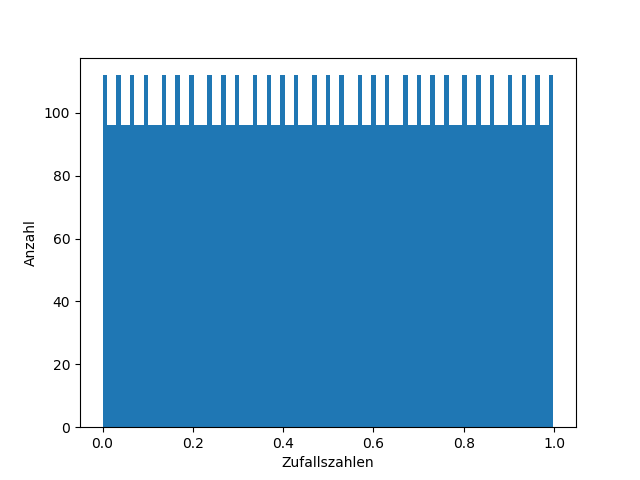
\includegraphics[width=0.6\textwidth]{plots/Zufallszahlen2b.png}
  \caption{Histogramm der gezogenen Zufallszahlen.}
  \label{fig:Hist2b}
\end{figure}
Das Ergebnis zeigt, dass der linear-kongruente Generator keine wirkliche Gleichverteilung
erzeugt, was ein \textit{guter} Zufallszahlengenerator tun sollte.
Die Höhe der einzelnen Spitzen ist dabei (minimal) vom Seed abhängig, allerdings
wird nie eine echte Gleichverteilung entstehen.
\subsection{Teil c)}
In den folgenden Abbildungen sind Paare und Tripletts nachfolgender Zahlen dargestellt.
\begin{figure}[H]
  \begin{subfigure}{0.5\textwidth}
   \centering
   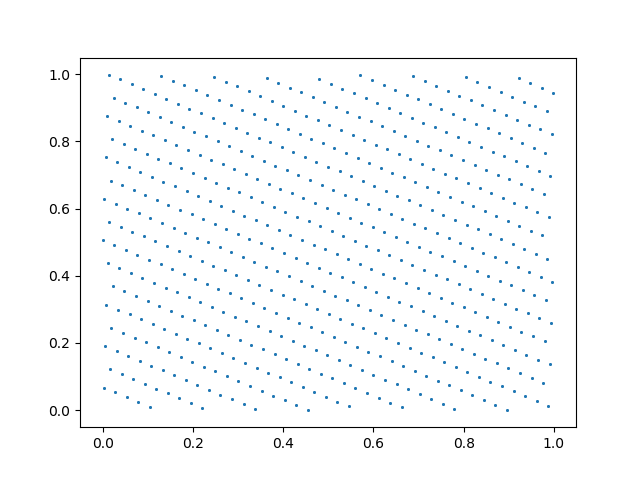
\includegraphics[width=0.8\textwidth]{plots/Paare2c.png}
   \label{fig:Paare2c}
\end{subfigure}
\begin{subfigure}{0.5\textwidth}
  \centering
  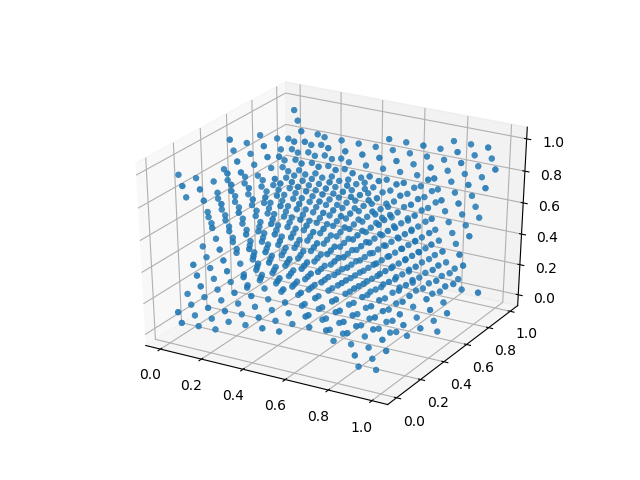
\includegraphics[width=0.8\textwidth]{plots/Triplets2c.png}
  \label{fig:Tripletts2c}
\end{subfigure}
\caption{Scatterplots der jeweils aufeinander folgenden Paaren und Tripletts für
          den linear-kongruenten Generator.}
\end{figure}
Es ist zu erkennen, dass die Punkte in beiden Scatterplots eindeutige Muster
erzeugen. In dem 2D-Plot zeigen sich Geraden, was auch nicht verwundet, da
die Vorschrift im Endeffekt eine Geradengleichung beschreibt, mit einem Versatz
durch die Modulo Operation. Dies wird Marsaglia Effekt genannt. Dies sollte ein
\textit{guter} Zufallszahlengenerator nicht zeigen.
\subsection{Teil d)}
Analog zum Teil c) wurden die Plots für den \textbf{numpy.random.unform()}-Generator
gemacht.
\begin{figure}[H]
  \begin{subfigure}{0.5\textwidth}
   \centering
   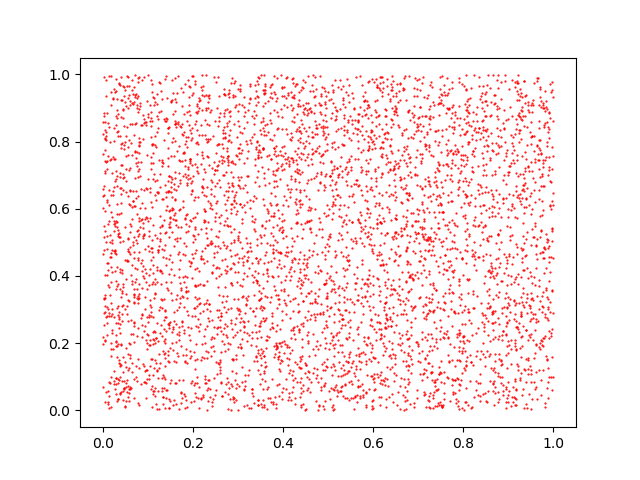
\includegraphics[width=0.8\textwidth]{plots/Paare2d.png}
   \label{fig:Paare2d}
\end{subfigure}
\begin{subfigure}{0.5\textwidth}
  \centering
  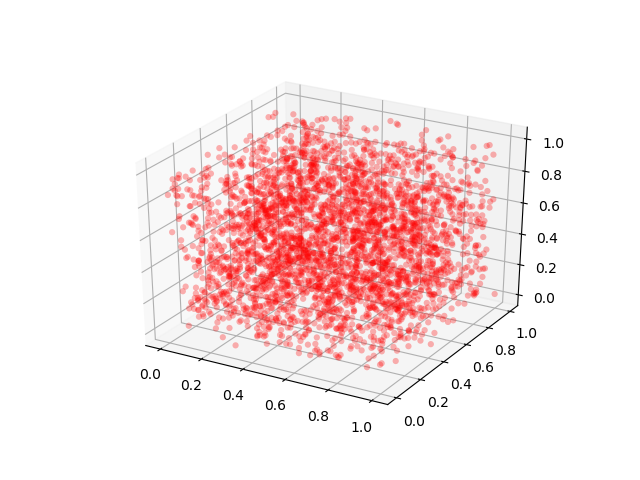
\includegraphics[width=0.8\textwidth]{plots/Triplets2d.png}
  \label{fig:Tripletts2d}
\end{subfigure}
\caption{Scatterplots der jeweils aufeinander folgenden Paaren und Tripletts für
den \textbf{numpy.random.unform()}-Generator.}
\end{figure}
Die Plots zeigen keine eindeutig erkennbare Muster zu erkennen, was darauf schließen lässt,
dieser Zufallszahlgenerator nicht auf dem Prinzio des linear kongruenten Generator beruht.
\subsection{Teil e)}
Ob der Generator aus Aufgabenteil a) den Wert $\frac{1}{2}$ erzeugen kann hängt sowohl
vom Wert des Seeds $x_0$ als auch von dem es Multiplikators $a$ ab. Um eine Kombination
zu finden, welche den Wert $\frac{1}{2}$ erzeugen kann, wird die Ausgangsgleichung
umgeformt. Wenn $x_1 = \frac{1}{2}$ sein soll, gilt:
\begin{align*}
  \frac{1}{2} &= (a\cdot x_0 +3)\%1024\\
  512 &= (a\cdot x_0 +3)\\
  509 &= a\cdot x_0 \\
  \frac{509}{a} &=x_0
\end{align*}
Ist nun der Wert von $a=1$ ist ein Startwert, der den Wert $\frac{1}{2}$
erzeugen kann, $x_0=509$. Dies ist eine Moglichkeit den Wert $\frac{1}{2}$ hat.
